\documentclass{article}
\usepackage[margin=1in]{geometry}
\usepackage{amsmath,amsthm,amssymb}
\usepackage{bbm,enumerate,mathtools}
\usepackage{tikz,pgfplots}
\usepackage{chessboard}
\usepackage[hidelinks]{hyperref}
\usepackage{multicol} % Problem 35

\newenvironment{question}{\begin{trivlist}\item[\textbf{Question.}]}{\end{trivlist}}
\newenvironment{note}{\begin{trivlist}\item[\textbf{Note.}]}{\end{trivlist}}
\newenvironment{references}{\begin{trivlist}\item[\textbf{References.}]}{\end{trivlist}}
\newenvironment{related}{\begin{trivlist}\item[\textbf{Related.}]\end{trivlist}\begin{enumerate}}{\end{enumerate}}


\begin{document}
\rating{3}{4}
A ``mod-$n$ XOR-triangle'' is a Pascal-like inverted triangle, where the first
row consists of numbers in $\{0, 1, \dots, n\}$, and the values in the cells
of the subsequent rows are computed as the sum (mod $n$) of the numbers
in the cells above them.

In the case of mod-$3$ XOR-triangles, if we additionally impose a constraint that
the boundary must be rotationally symmetric, some of the resulting triangles
appears to have emergent ``central circles'' reminiscent of the
``Arctic circles'' that appear in lozenge and domino tilings.

\begin{figure}[ht!]
  \centering
  \noindent
  \begin{tikzpicture}

  \end{tikzpicture}
  \definecolor{pink1}{rgb}{1,0.8,0.9}
  \definecolor{blue2}{rgb}{0.8,0.9,1}
  \begin{tikzpicture}[scale=1.1]
    \foreach \a/\b/\n/\tc/\c in {
      0/1/0/white/black, 1/1/0/white/black, 2/1/1/black/pink1, 3/1/0/white/black, 4/1/1/black/pink1, 5/1/0/white/black, 6/1/0/white/black,
      0/2/0/white/black, 1/2/1/black/pink1, 2/2/1/black/pink1, 3/2/1/black/pink1, 4/2/1/black/pink1, 5/2/0/white/black,
      0/3/1/black/pink1, 1/3/2/black/blue2, 2/3/2/black/blue2, 3/3/2/black/blue2, 4/3/1/black/pink1,
      0/4/0/white/black, 1/4/1/black/pink1, 2/4/1/black/pink1, 3/4/0/white/black,
      0/5/1/black/pink1, 1/5/2/black/blue2, 2/5/1/black/pink1,
      0/6/0/white/black, 1/6/0/white/black,
      0/7/0/white/black}{
      \draw[
        fill=\c,
        xshift=\b*0.433cm + \a*0.866cm,
        yshift=\b * -0.75cm
      ]
        (30:0.5)--(90:0.5)--(150:0.5)--(210:0.5)--(270:0.5)--(330:0.5)--cycle
      ;
      \node[text=\tc] at (\b*0.433 + \a*0.866, \b * -0.75) {$\n$};
    }
  \end{tikzpicture}
  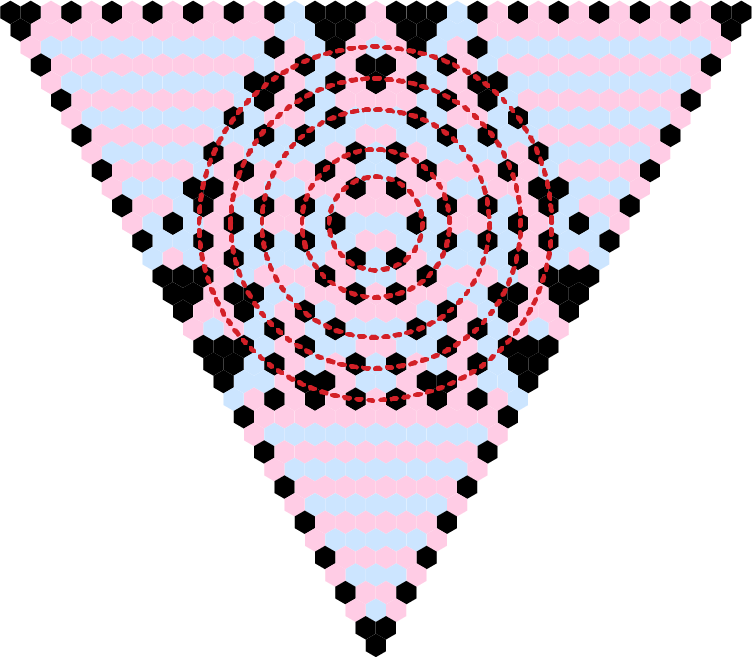
\includegraphics[width=20em]{assets/124_problem/Triangle37_5_circles.png}
  \caption{
    An illustration of the construction of a mod 3 sum triangle, and some
    candidates for central circles for an example of a triangle with $37$ cells
    per side.
  }
\end{figure}
\begin{figure}[ht!]
  \centering
  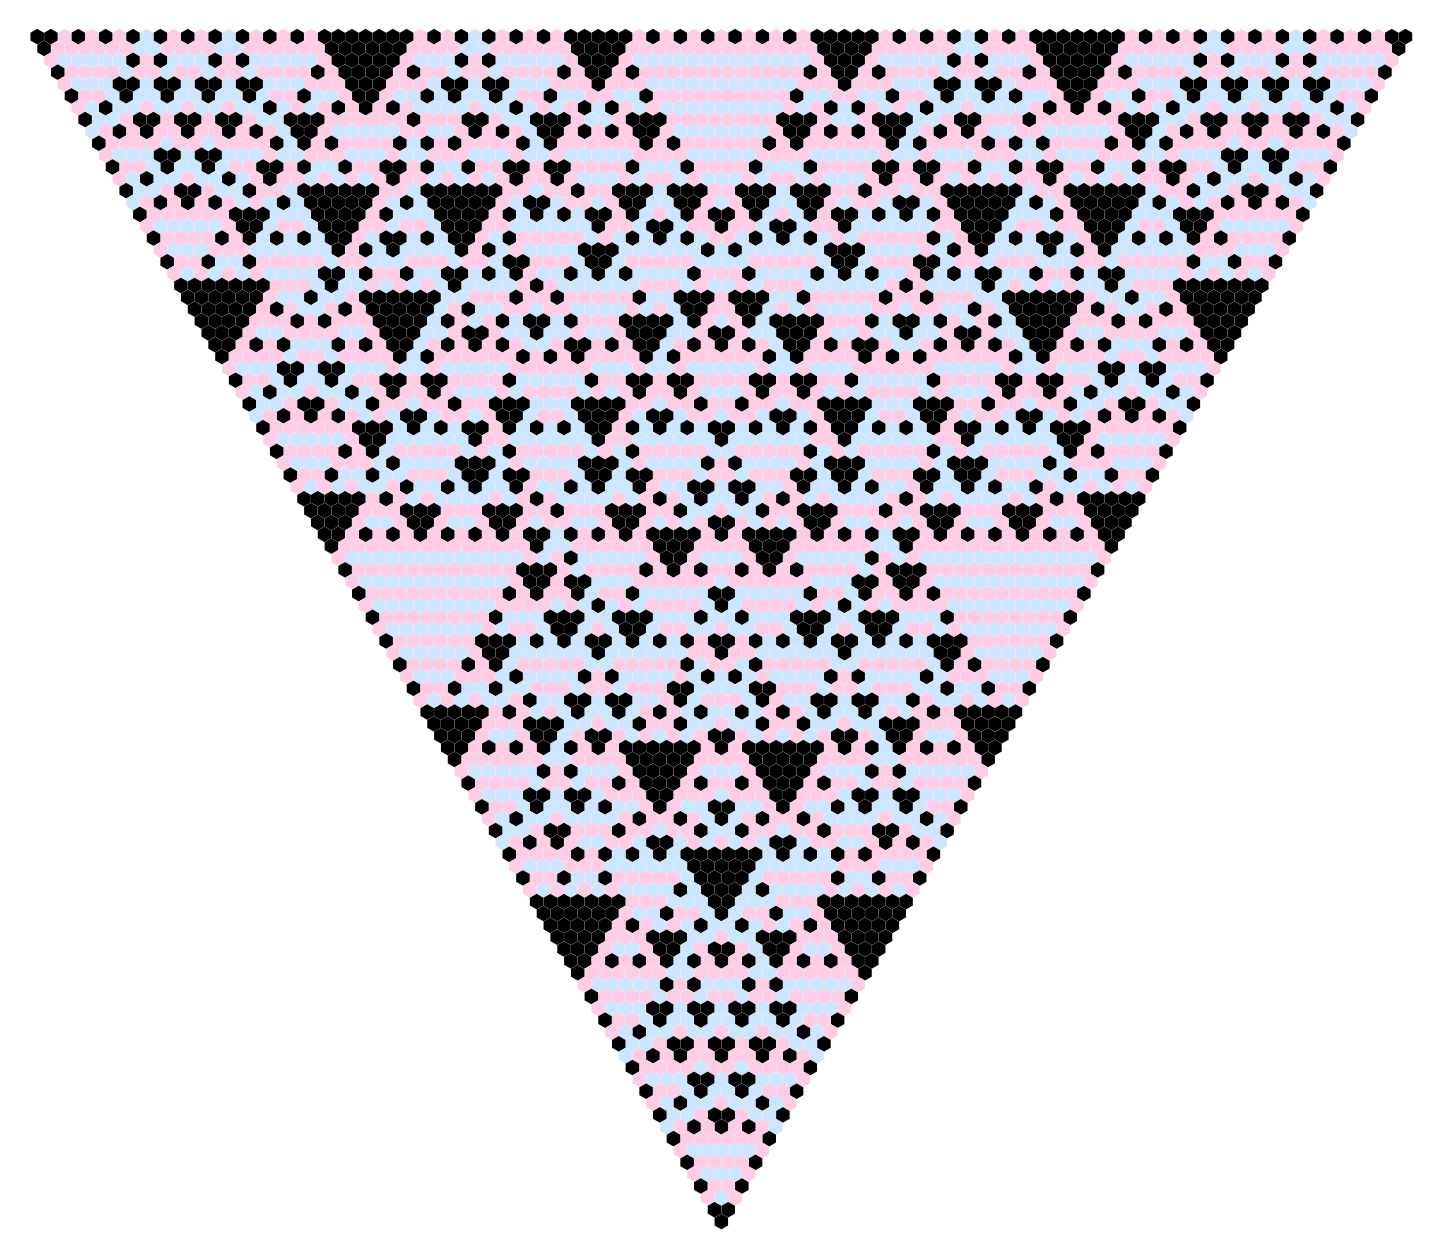
\includegraphics[width=10em]{assets/124_problem/triangle101_1.png}
  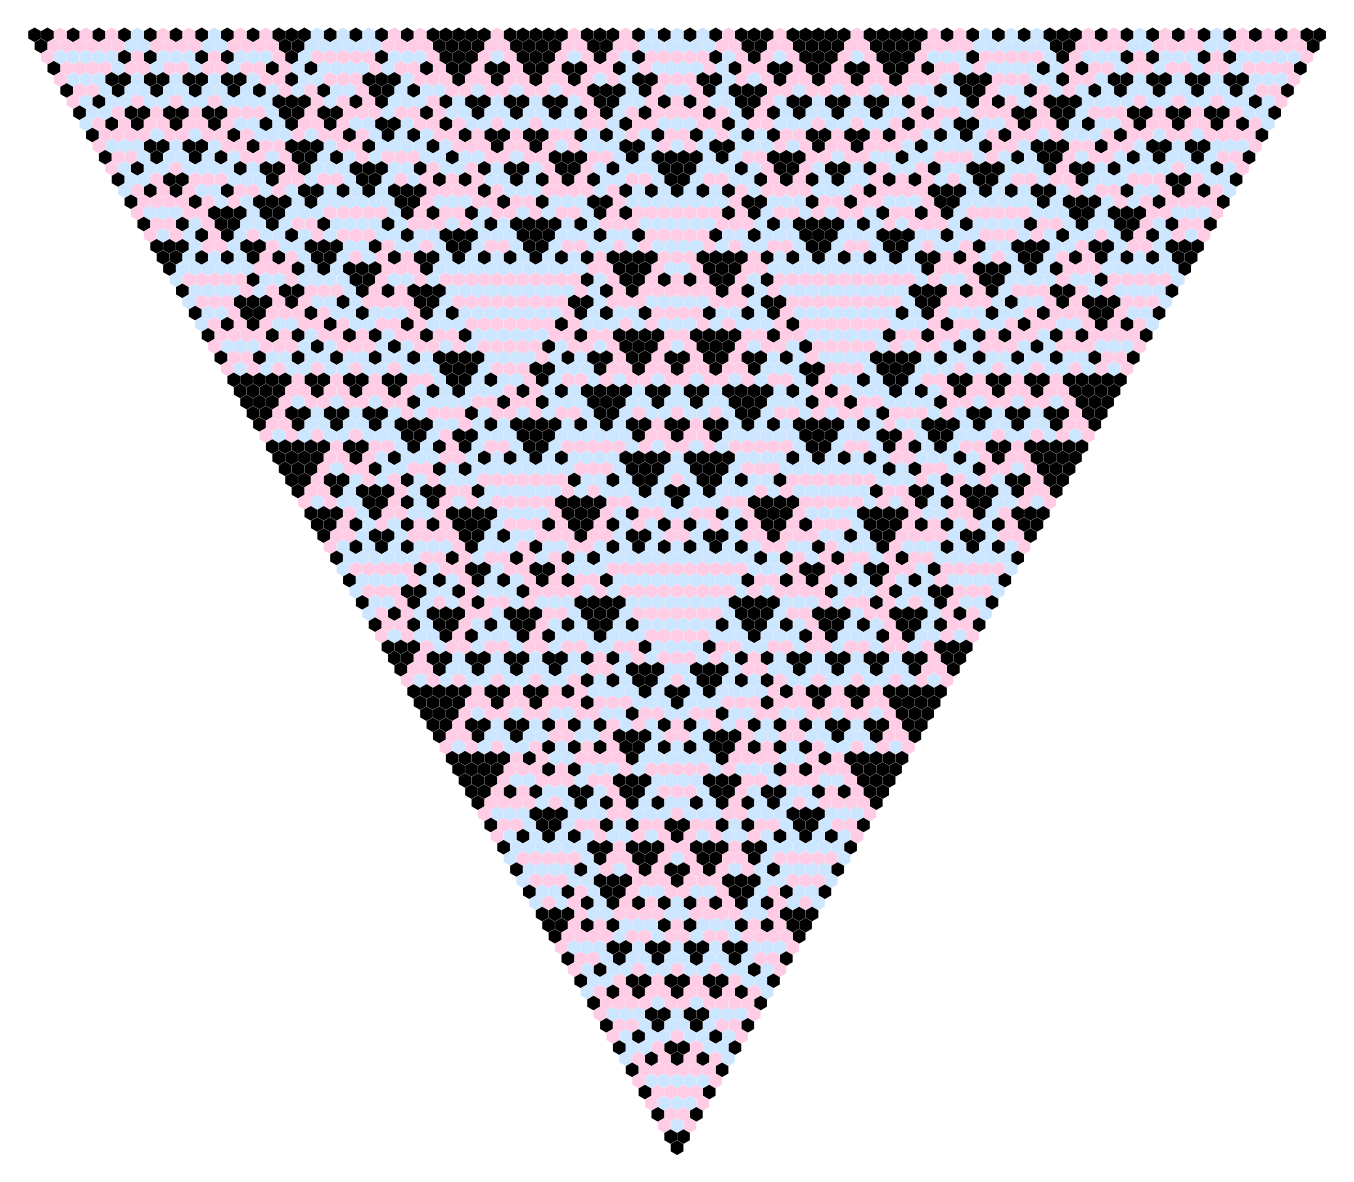
\includegraphics[width=10em]{assets/124_problem/triangle101_2.png}
  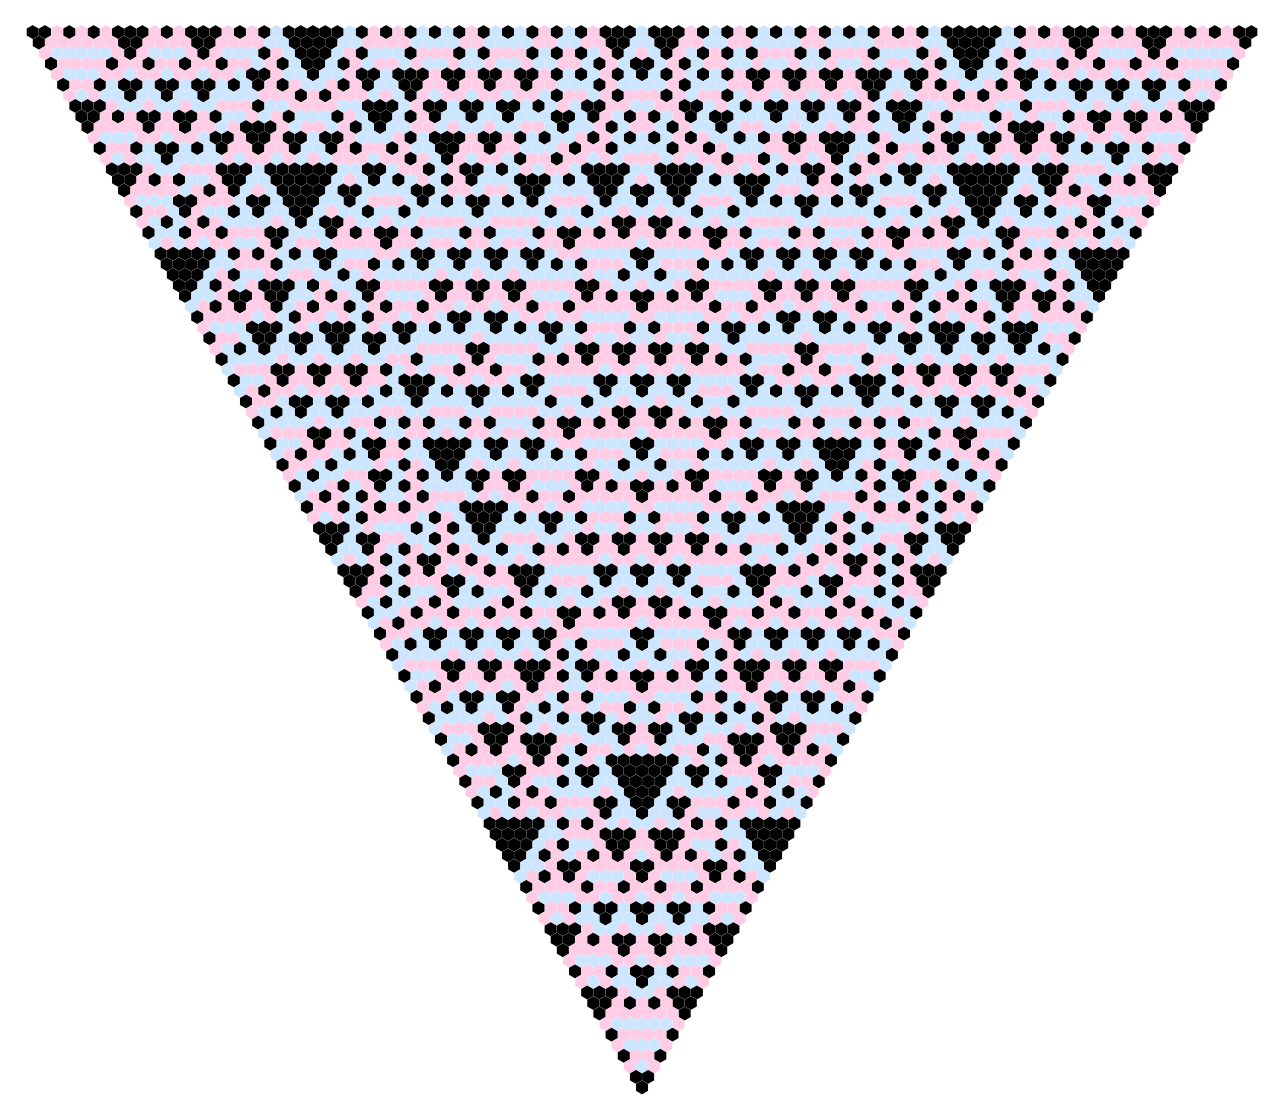
\includegraphics[width=10em]{assets/124_problem/triangle101_3.png}
  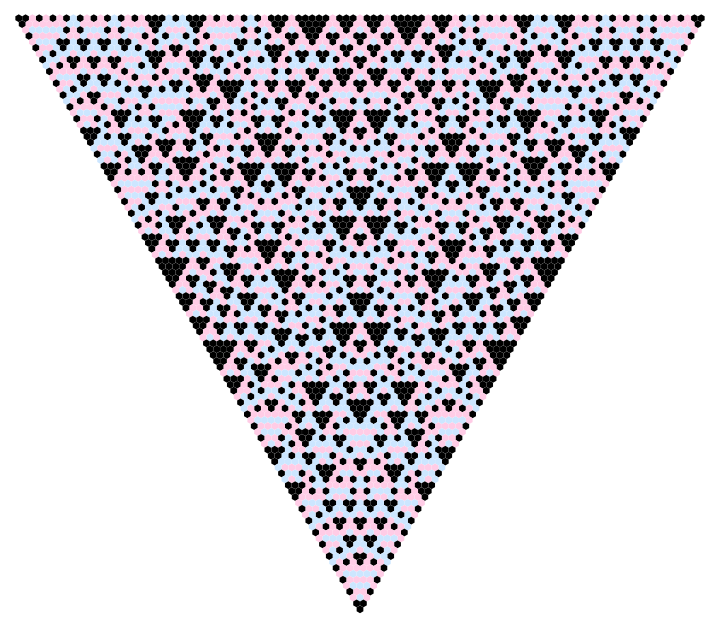
\includegraphics[width=10em]{assets/124_problem/triangle101_4.png}
  \caption{Four more examples of triangles that appear to have central circles}
\end{figure}

\begin{question}
  Are these central circles in mod-$3$ XOR-triangles optical illusions or
  coincidences?
  If not, what's a mathematical explanation for why they exist?
\end{question}

\begin{related}
  \item What about other moduli?
  \item Why does the boundary condition cause the black ($0$) cells to be
  symmetric with respect to the dihedral group of the triangle?
  \item Can we create meaningful analogs where the shape is a square,
  tetrahedron, or another shape instead of a triangle?
\end{related}

\begin{references}
  \item \url{https://math.stackexchange.com/q/4088671/121988}
\end{references}
\end{document}
